\chapter{Evaluation}
In this chapter, insights emanating from each queue's evaluation is compared
with findings from their seminal works; each queue's performance is compared, 
together with explanations as to why and what makes a queue superior to another.

\section{Workload under one thread}

\begin{figure}[!ht]
    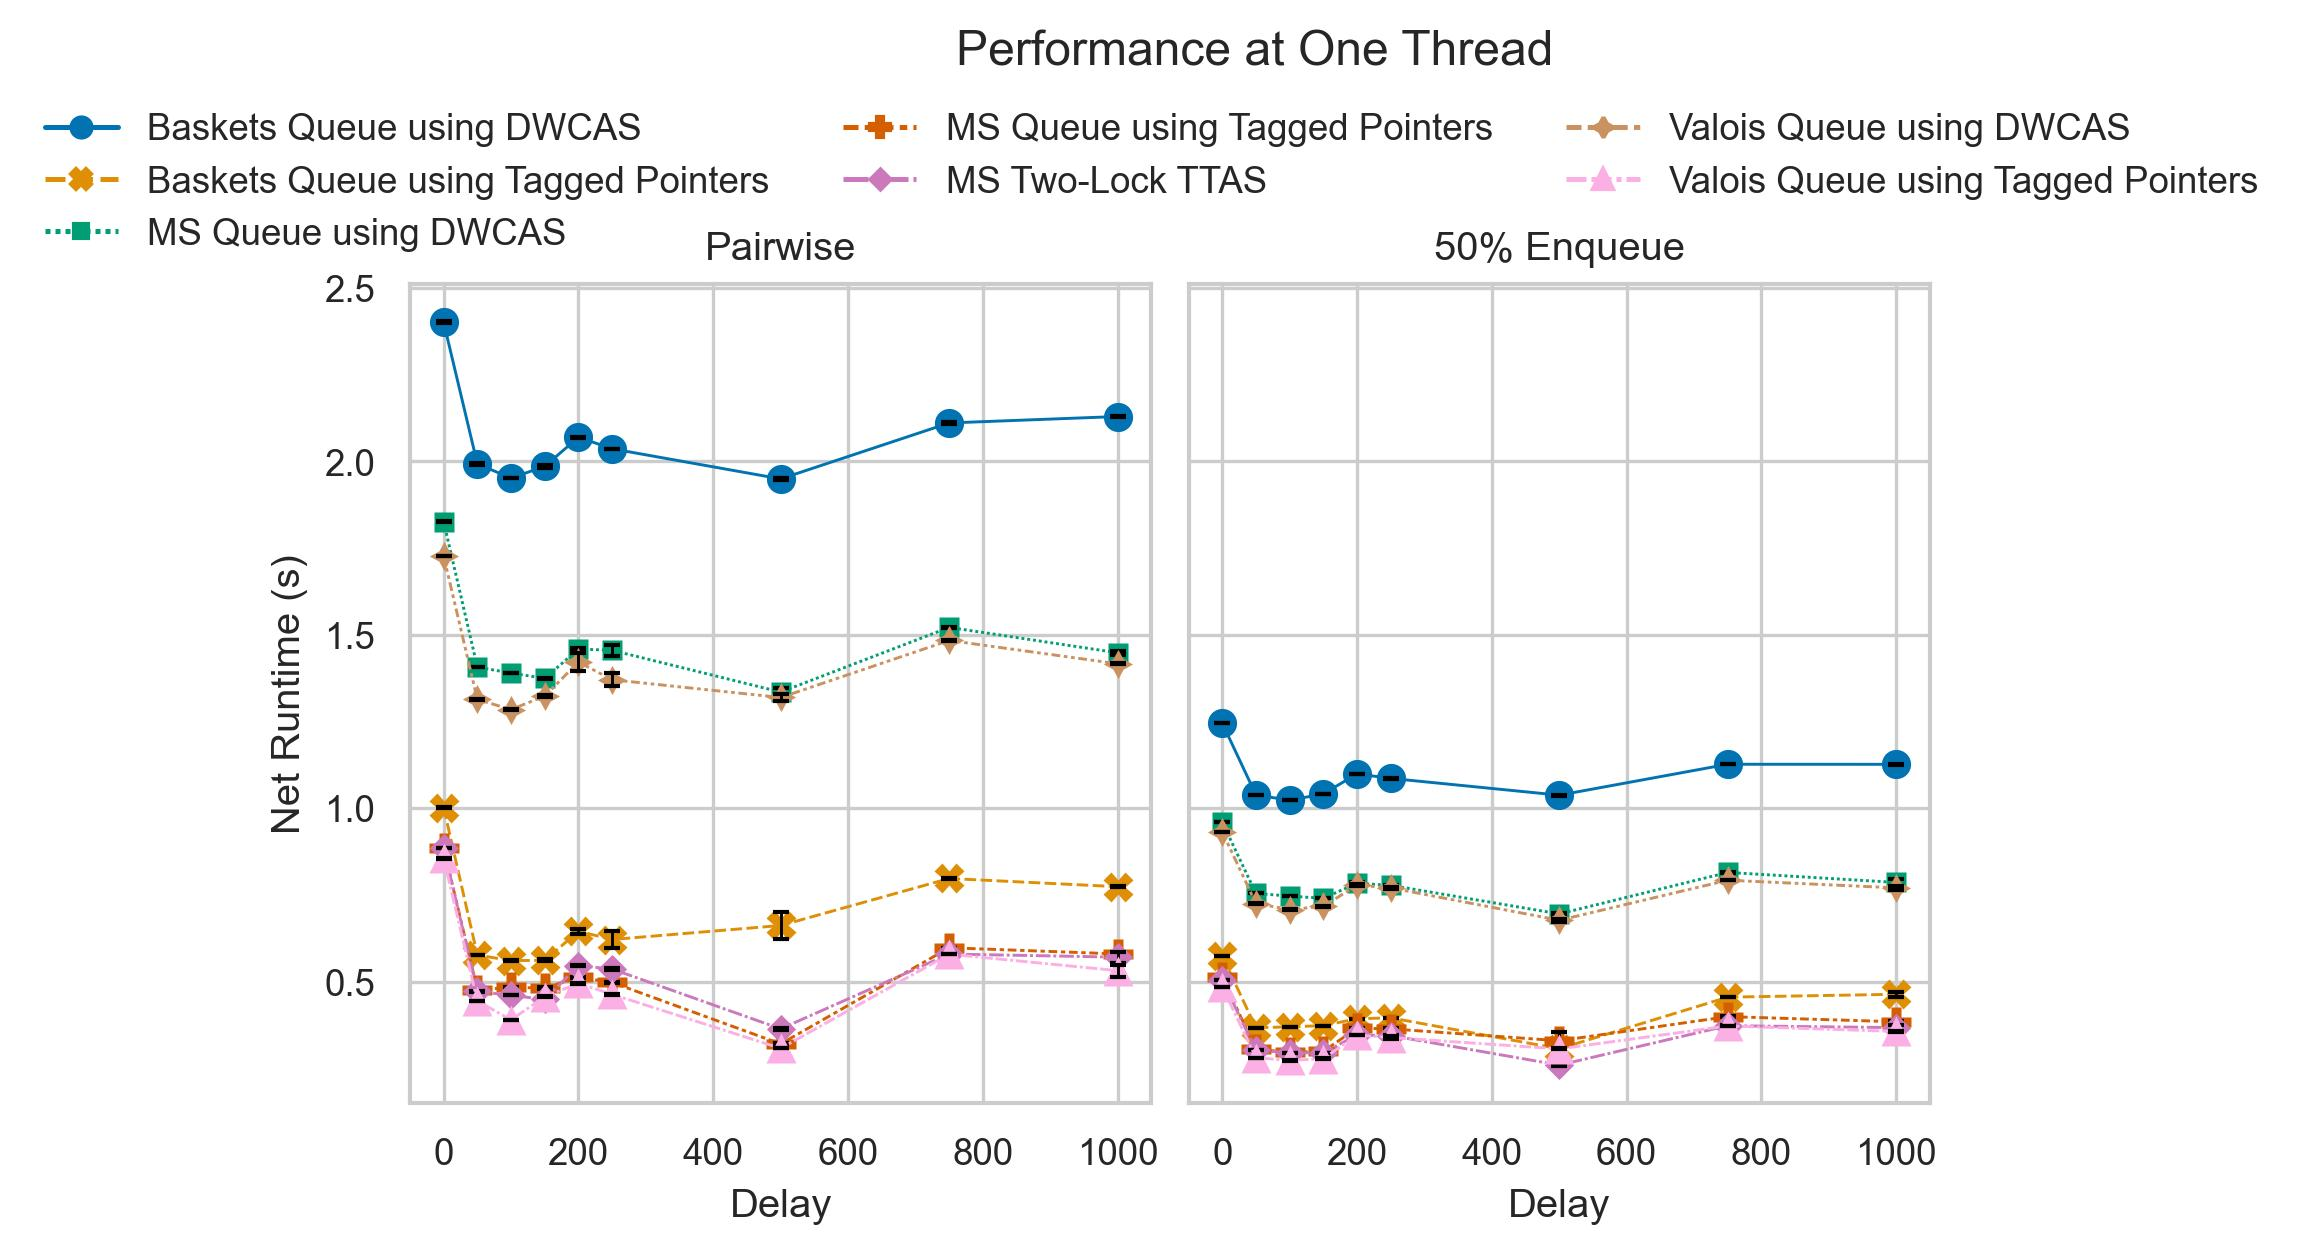
\includegraphics[width=1\textwidth]{plots/delay_thread_1.jpg}
    \caption{The pairwise and the 50\% benchmarks on the left and right respectively.}
    \label{fig:perf_1_thread}
\end{figure}

The sequential latency of a queue is determined by its algorithmic
complexity~\citep{valois1995datastructures}. Contention-reducing mechanisms,
such as thread helping, are not triggered under single threaded workloads, as
they rely on failed Compare-and-Swaps, adding extra overhead through the
computation of predicates. Figure \ref{fig:perf_1_thread} shows the performance
of each queue in a single threaded workload; Nonblocking queues using
tagged pointers perform twice as fast as their DWCAS counterparts.  
Most queues achieve optimal performance at a delay of 500 nanoseconds, with
the exception being the baskets queue using tagged pointers, due to its more
elaborate contention-reducing mechanisms.

\section{Workload under two threads}
Similar to \citep{michael1996simple,hoffman2007baskets,ladan2008optimistic},
under a workload of two threads, a significant degradation in performance can
be observed. \citeauthor{michael1996simple} notes that as each queue's head and
tail are shared across two processors, cache misses are more frequent. Figure
\ref{fig:perf_deg_1_thread} shows the ratio of time taken between two-threaded
and single threaded workloads, which represent the magnitude of performance
degradation between both workloads. Queues using tagged pointers tend to
experience higher contention, consequently leading to a harsher degradation in
performance; in support of this claim, the Baskets Queue using Tagged pointers
with zero delay was \textbf{61\%} more likely to re-attempt an enqueue\footnote{This metric was gathered by
incrementing an integer (found in thread local storage) every time it repeated
anything past line \emph{E03} of the Baskets Queue.} than its DWCAS counterpart.

\begin{figure}[!ht]
    \centering
    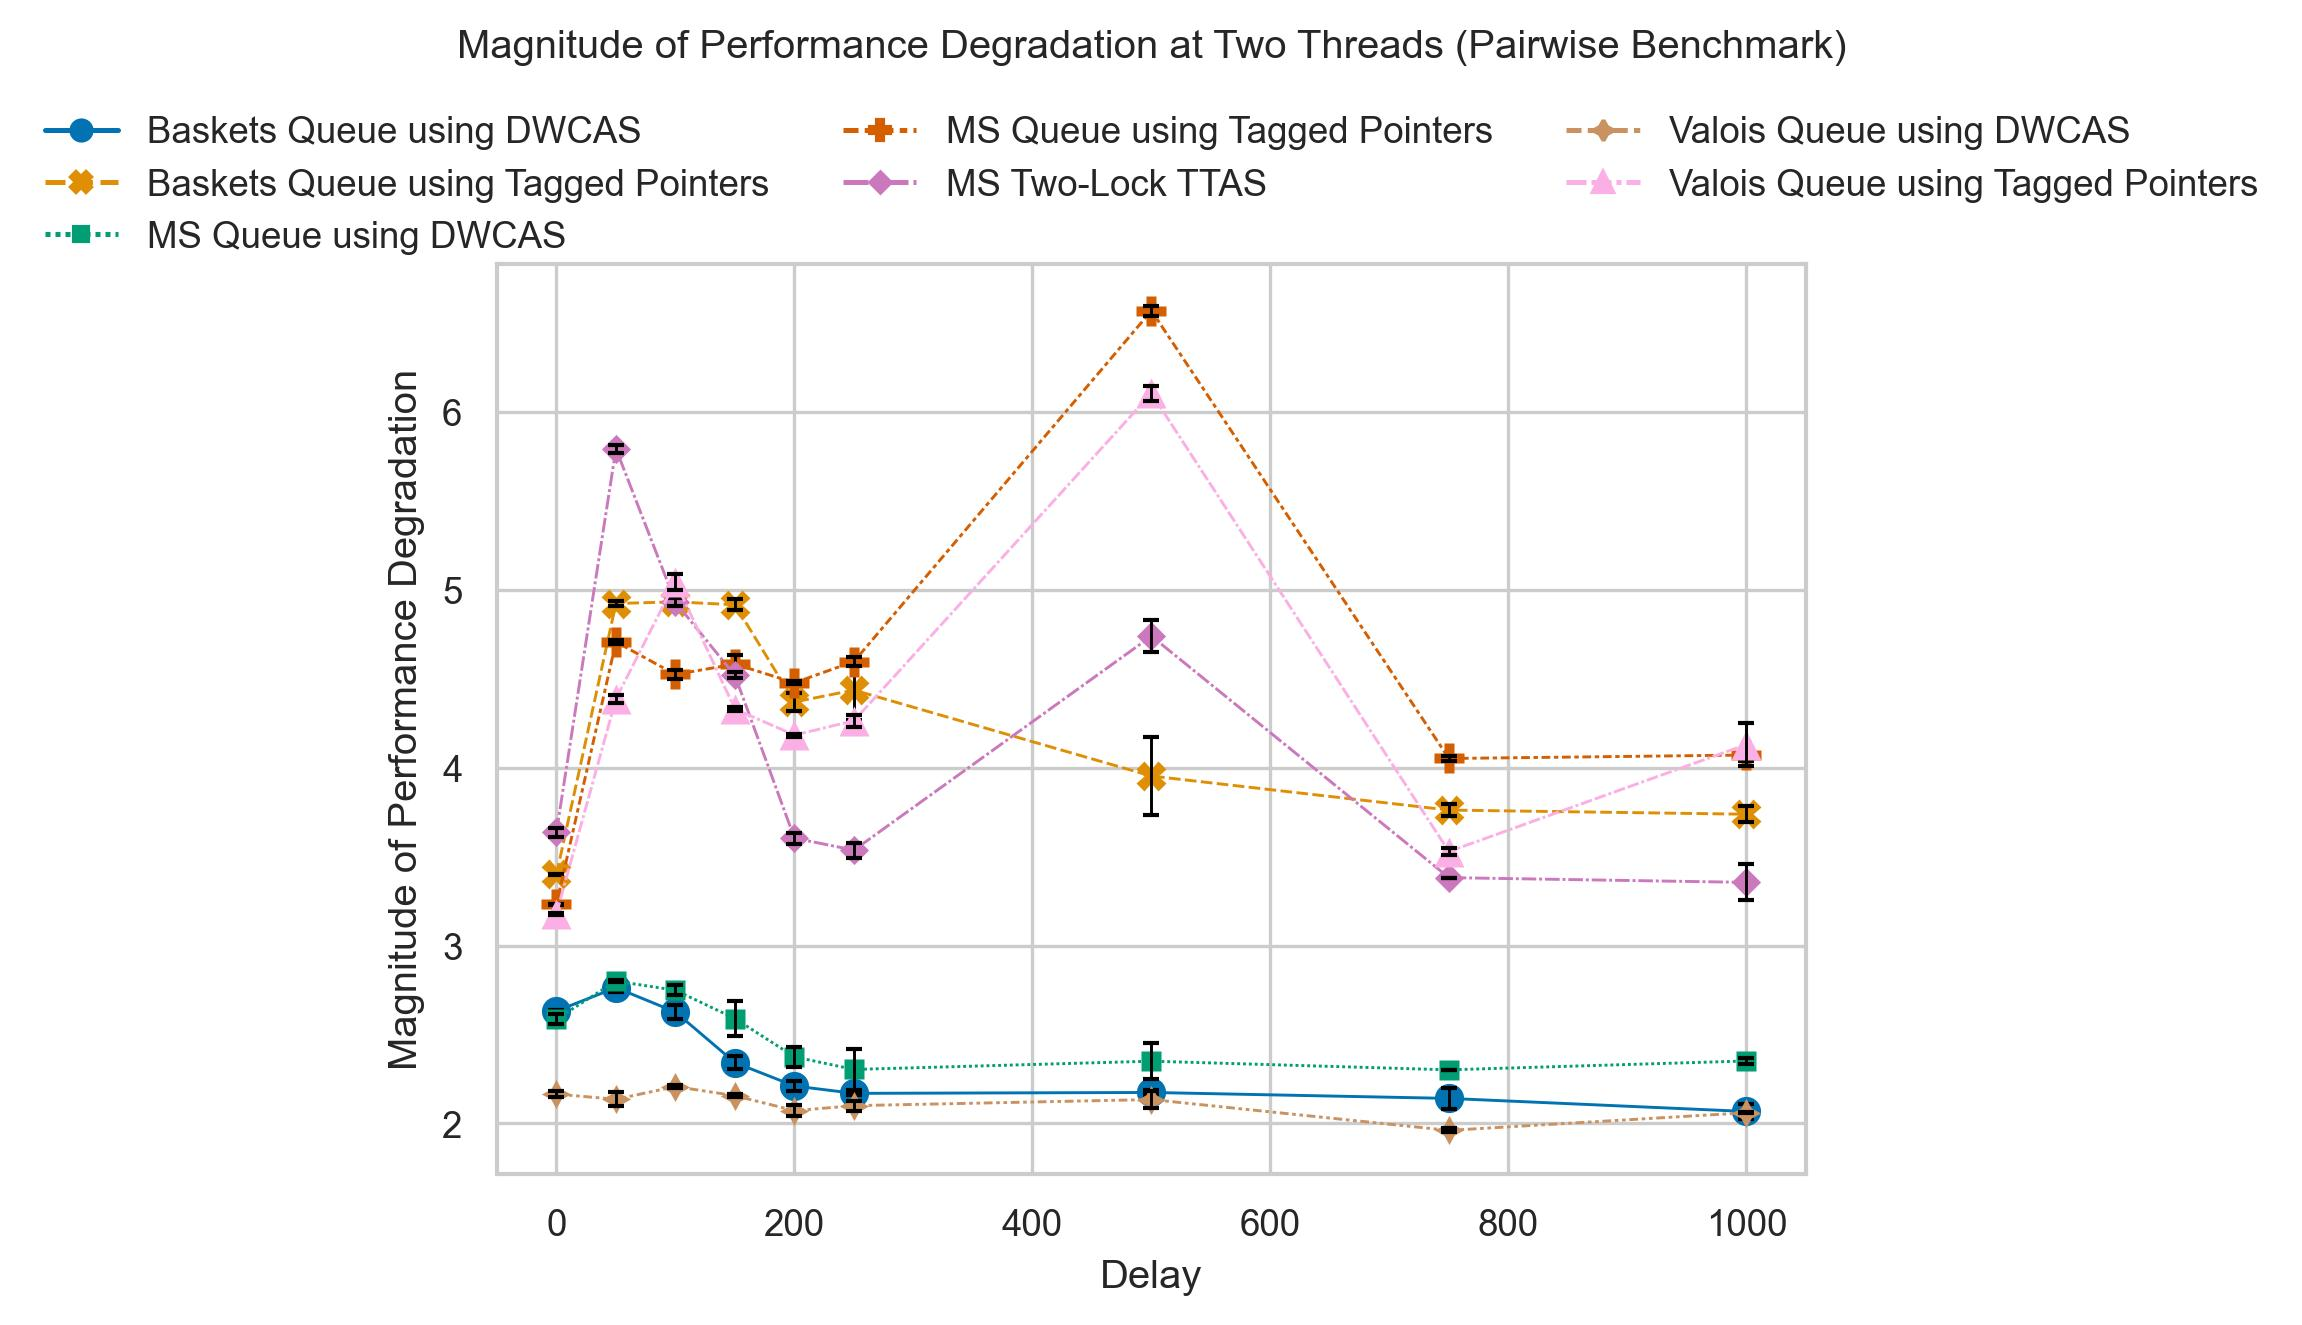
\includegraphics[width=1\textwidth]{plots/speedup_enqueue_dequeue_1.jpg}
    \caption{The magnitude of performance degradation between single and two-threaded workloads.}
    \label{fig:perf_deg_1_thread}
\end{figure}

\begin{figure}[!ht]
    \centering
    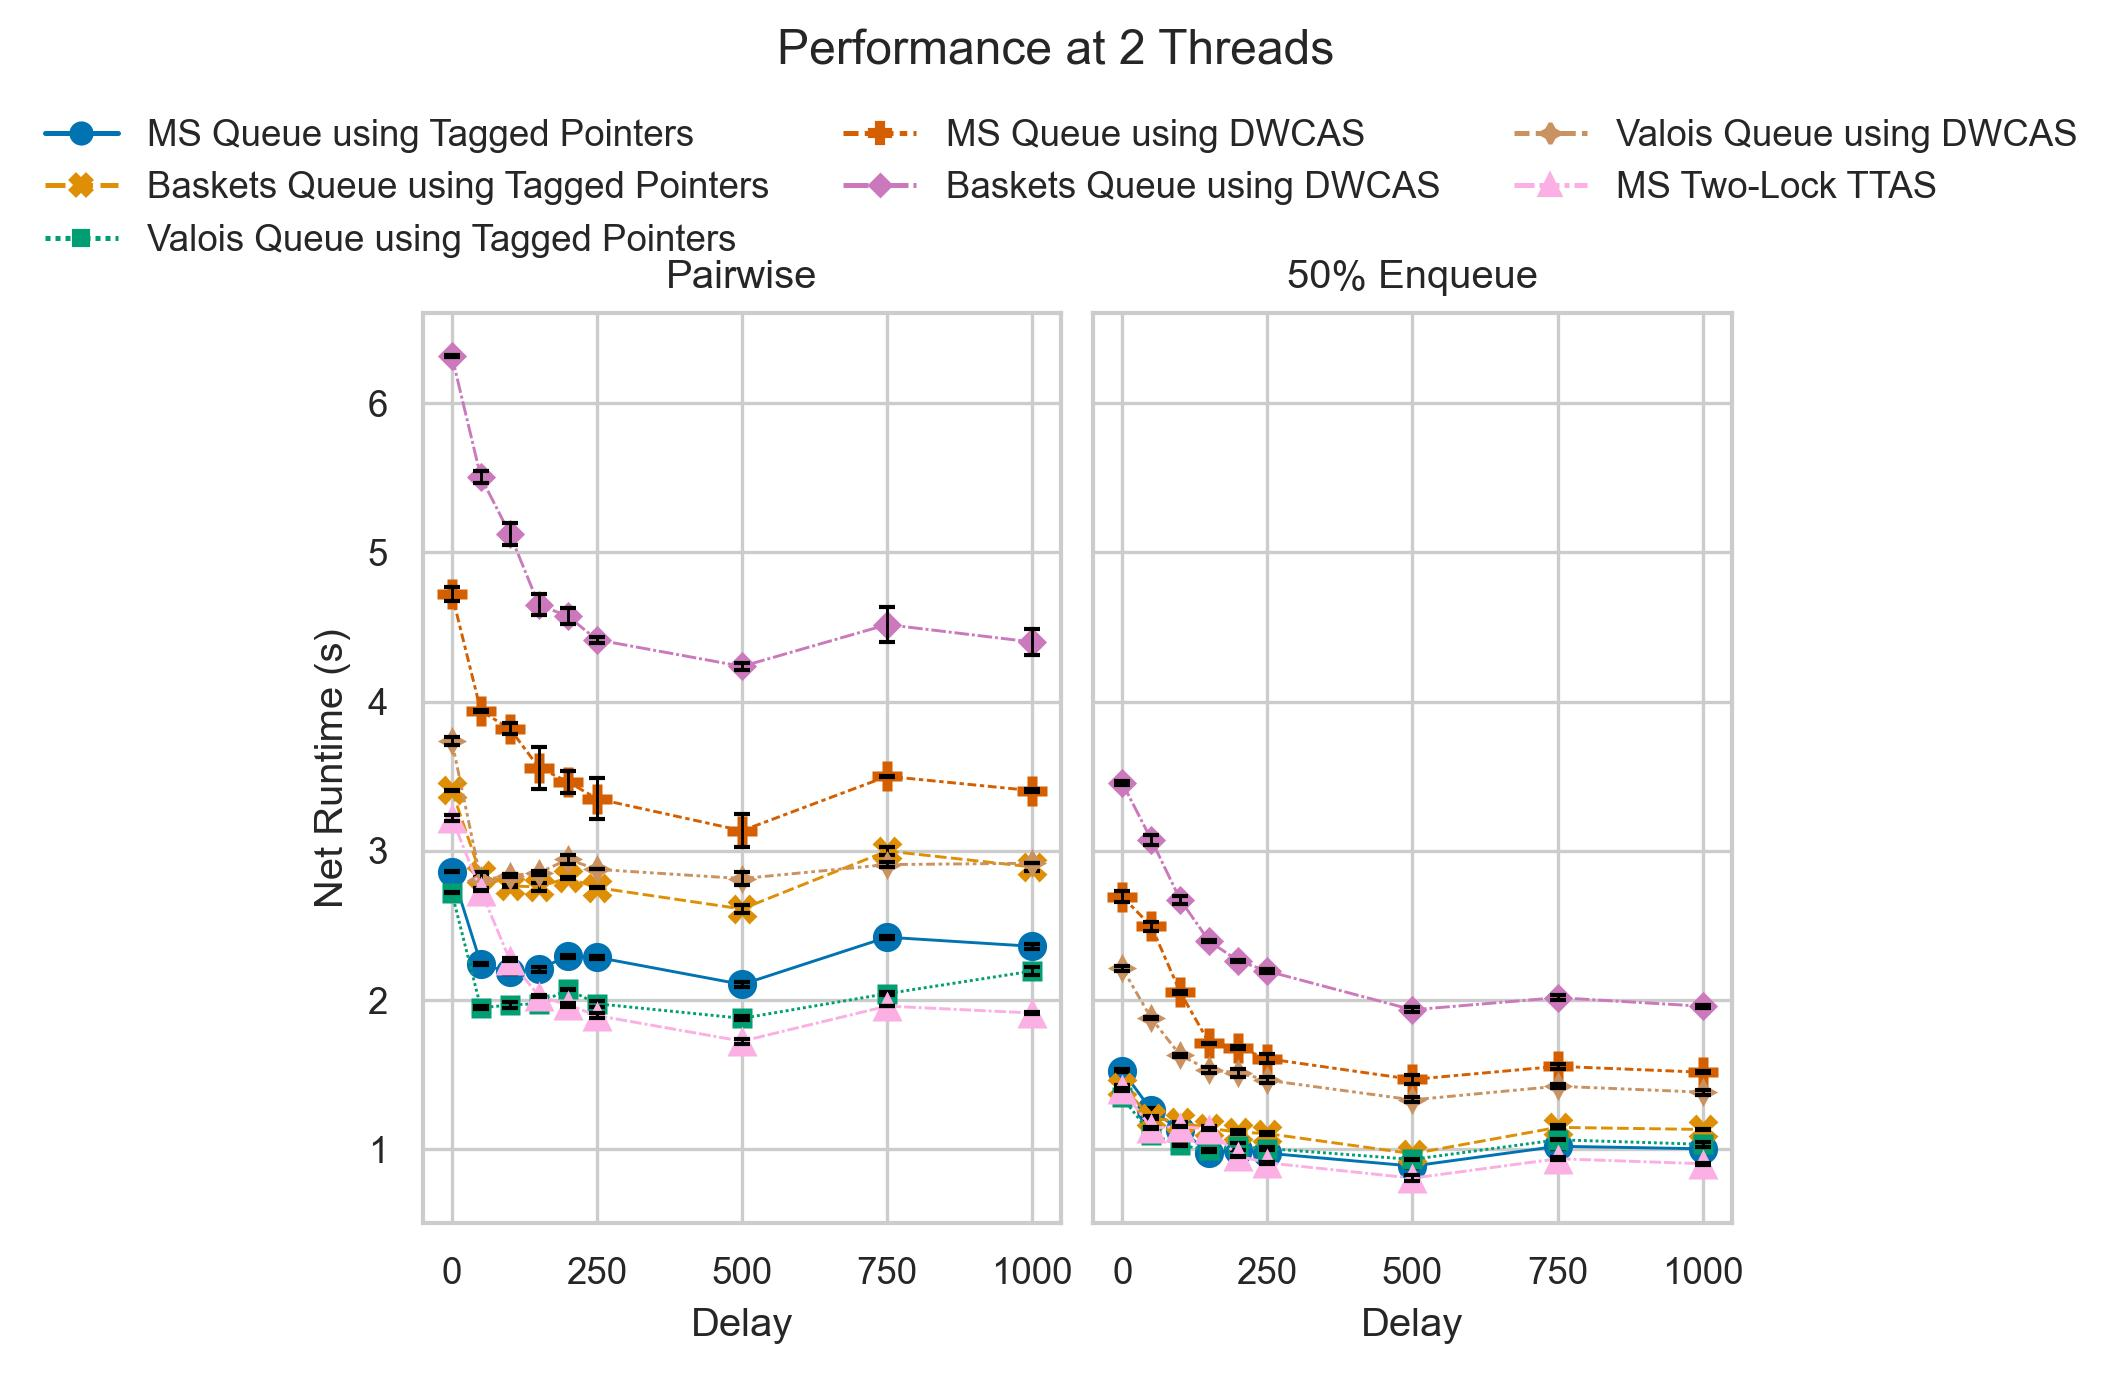
\includegraphics[width=1\textwidth]{plots/delay_thread_2.jpg}
    \caption{The pairwise and the 50\% benchmarks on the left and right respectively.}
    \label{fig:perf_2_thread}
\end{figure}

At delays greater than 200 nanoseconds, the two-lock queue exhibits the best
performance; nonblocking queues using tagged pointers remain competitive in
low-contention scenarios. 

The performance of \citeauthor{valois1994queues}' queue in this study highly
conflicts with that of \citep{michael1996simple}. Although a queue without a
memory reclamation scheme may share a common algorithm with one that has, it
does not imply that they are algorithmically equivalent, making their
performance unconnected; as this study does not include memory reclamation
schemes in its implementations, valid comparisons cannot be made with
~\citep{michael1996simple}'s results of \citeauthor{valois1994queues}' queue,
however, insights may still be inferred.
\citeauthor{michael1996simple}\textemdash conveniently\textemdash fail to
disclose that memory reclamation overheads were excluded from the reported
performance of the MS-queue, leading to biased comparisons against other
queues.

One may hypothesize \citeauthor{valois1994queues}' queue fitted with the \emph{safe read}
protocol leads to a horribly inefficient algorithm, as each enqueueing thread
is required to traverse part of the linked list, incurring a high number of
cache misses, since a reference counter has to be modified twice with each
traversal (once to reclaim a node, and another to release it).

\section{Workload Under Three Threads}
In \citep{ladan2008optimistic,michael1996simple,hoffman2007baskets},
a minor improvement in performance under three threads is observed;
\citeauthor{michael1996simple} link the boost in performance to the fewer
iterations per thread, combined with a cache miss rate similar to that under
two threads.

\begin{figure}[!ht]
    \centering
    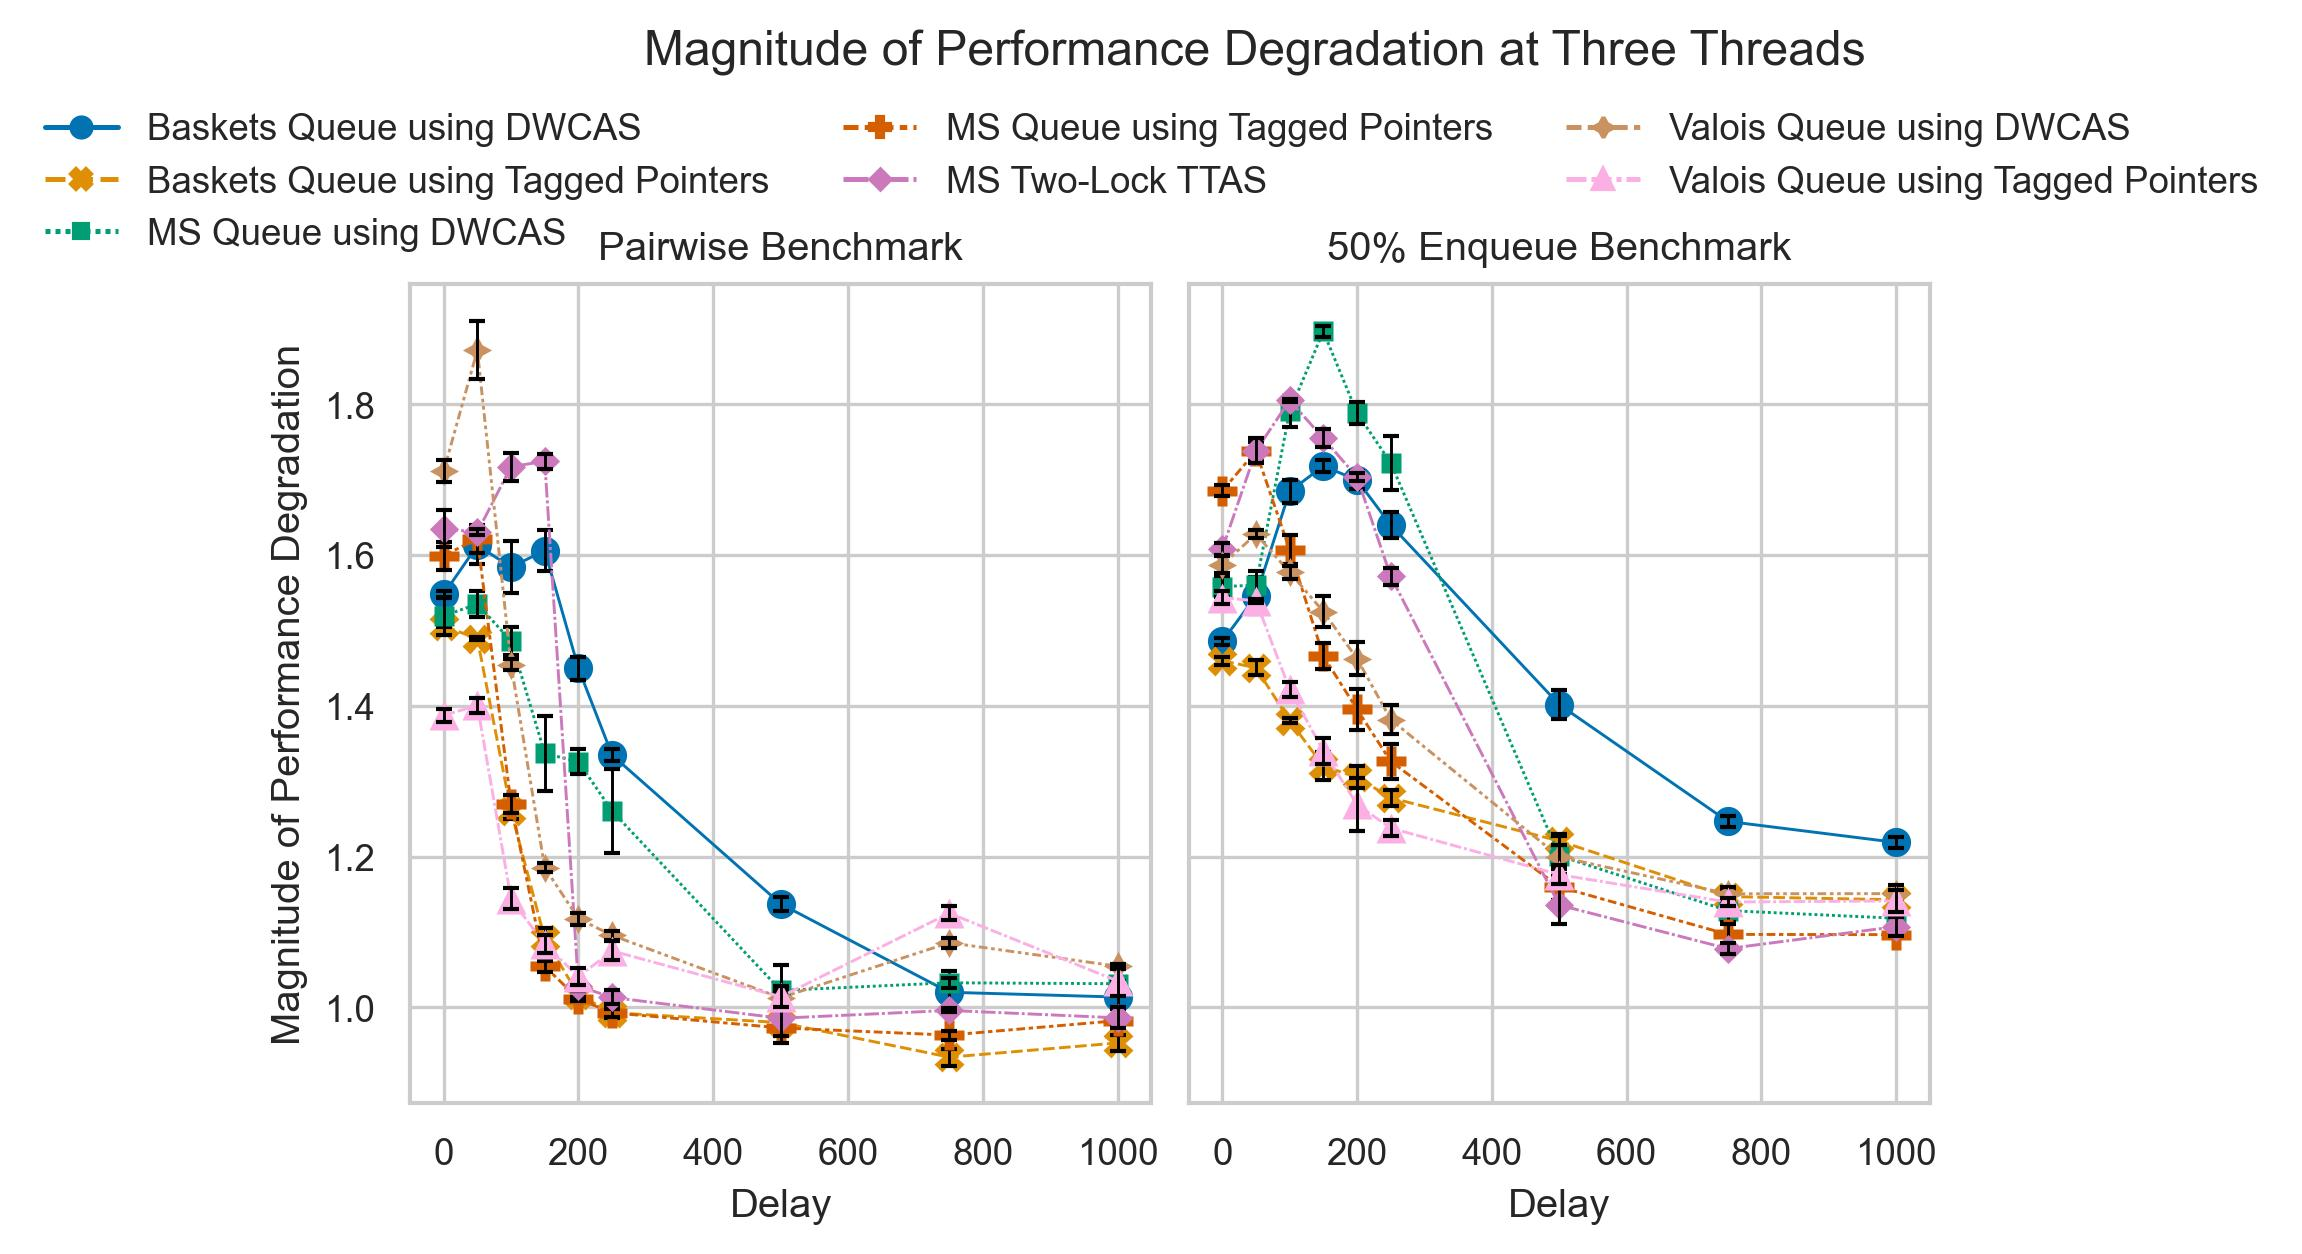
\includegraphics[width=1\textwidth]{images/plots/speedup_2.jpg}
    \caption{The pairwise and the 50\% benchmarks on the left and right respectively.}
    \label{fig:perf_deg_2_thread}
\end{figure}

Figure~\ref{fig:perf_deg_2_thread} shows that at specific delays\textemdash
speedups of up to \textbf{6.591\%} can be obtained.
\citeauthor{michael1996simple} observe speedups of a factor less than
$\frac{1}{3}$~\citep{michael1996simple}, which is far more drastic than that
observed in \citep{ladan2008optimistic, hoffman2007baskets} and this study. The
50\% enqueue benchmark does not exhibit any speedups, further highlighting the
effects of a benchmark's artificiality on the validity of its results.

\begin{figure}[!ht]
    \centering
    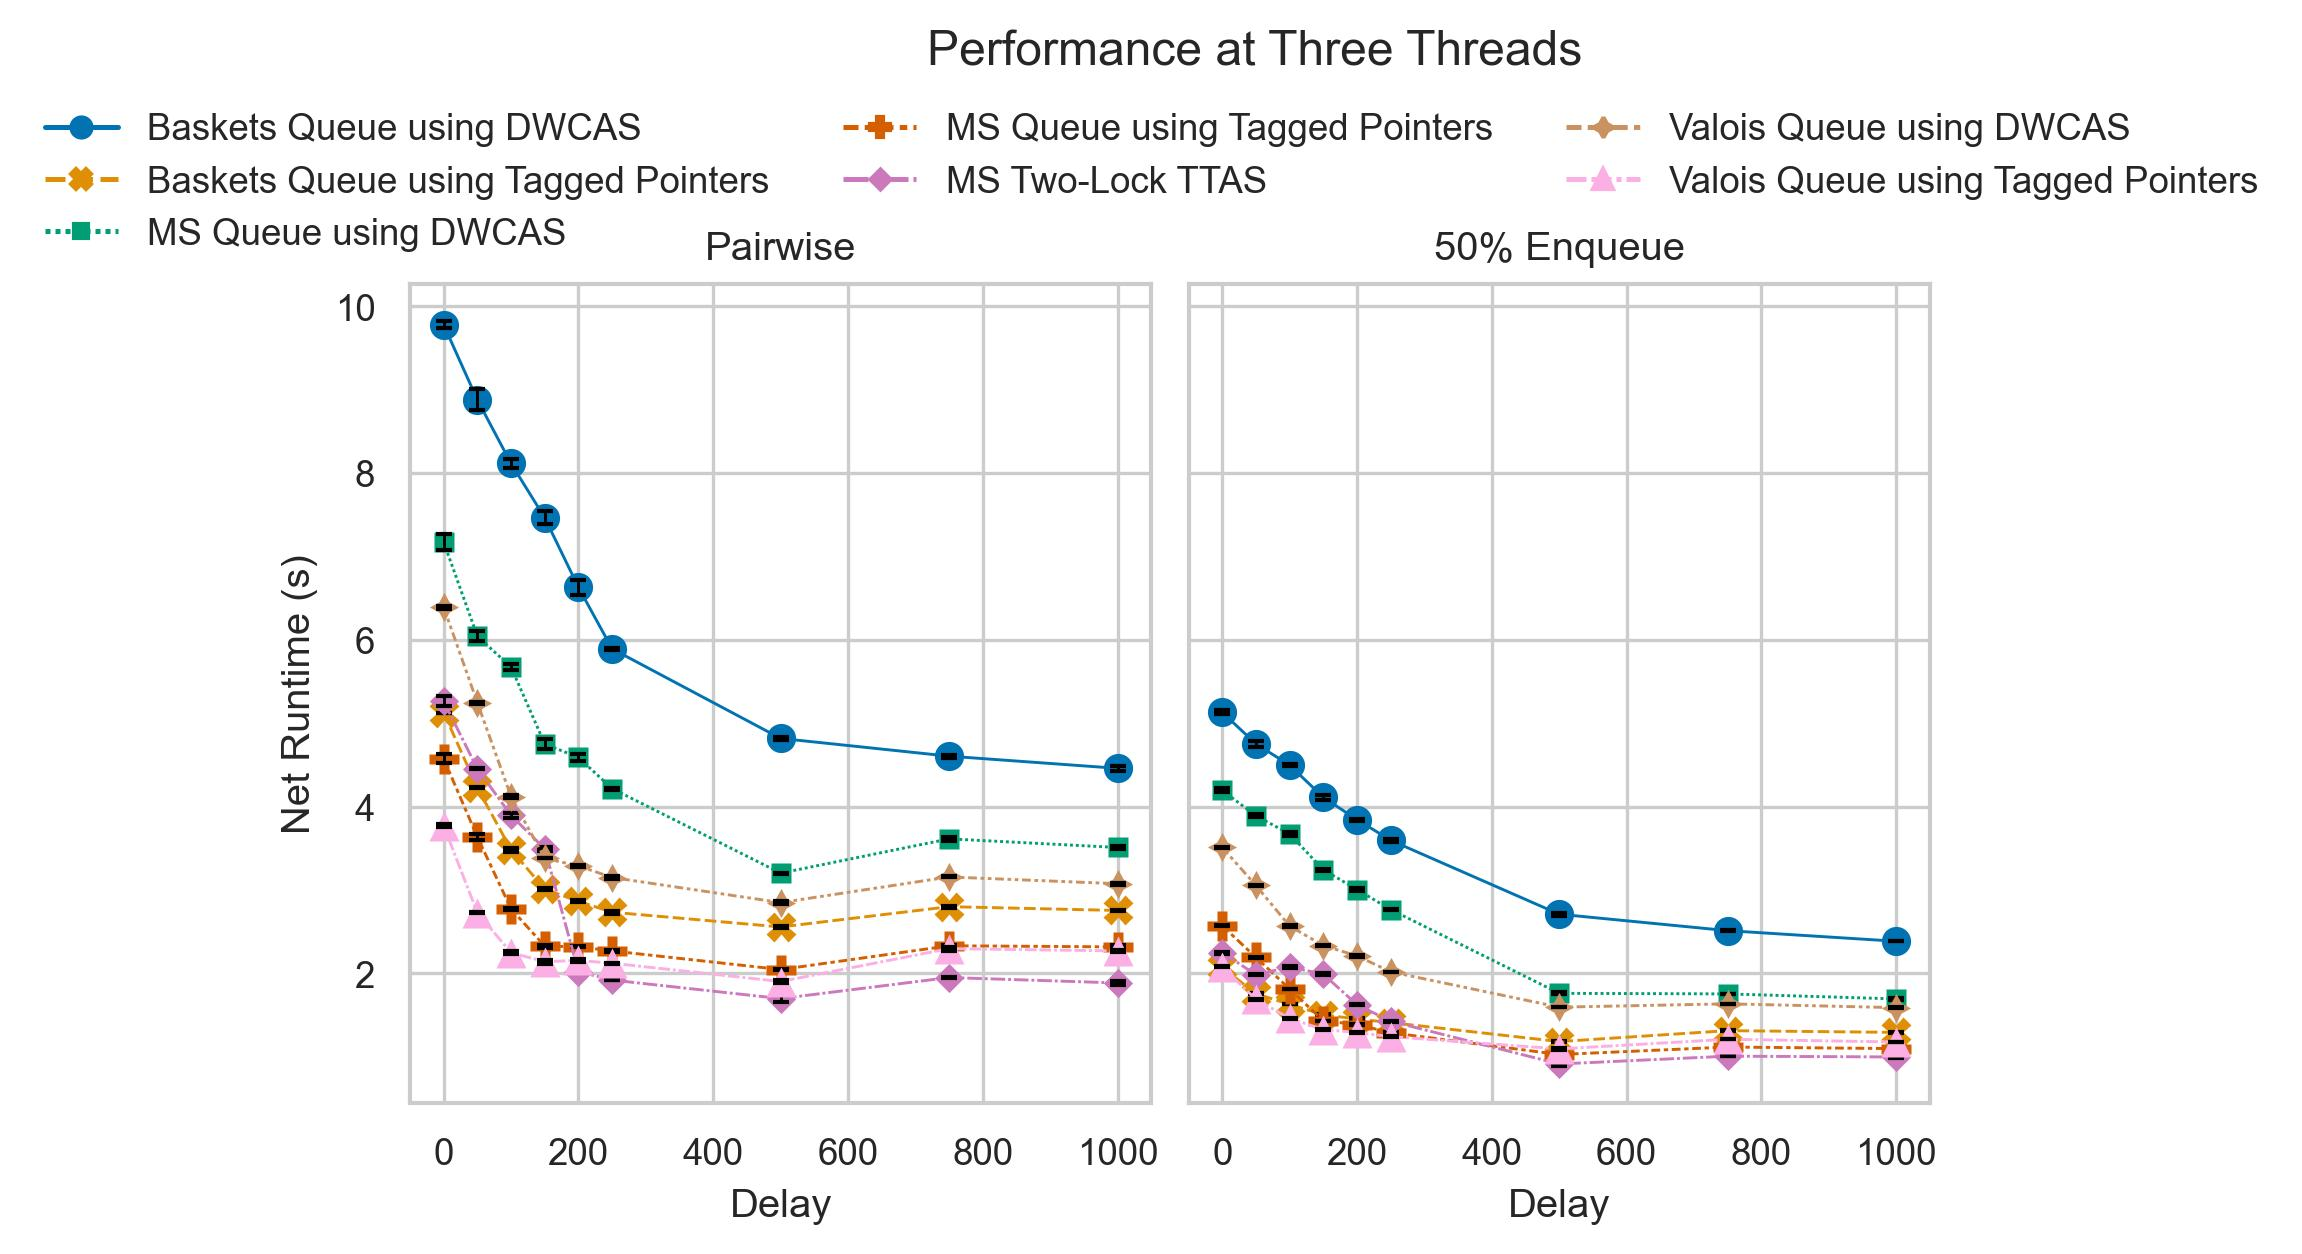
\includegraphics[width=1\textwidth]{images/plots/delay_thread_3.jpg}
    \caption{The pairwise and the 50\% benchmarks on the left and right respectively.}
    \label{fig:perf_3_thread}
\end{figure}

Up to delays of 150 nanoseconds, every non-blocking queue using tagged
pointers significantly outperforms the two-lock queue (MS queue is
\textbf{33.412\%} times faster than the two-lock queue at 150 nanoseconds of
delay), however, as contention drops, the two-lock queue tends to become more
favourable. The MS-queue consistently outperforms the Baskets queue by at least
\textbf{10.778\%}. As the degree of contention under three threads is
higher than that at two threads, the performance penalty in using higher delays
is reduced.

\section{Workload Under Four Threads\label{sec:workload_four_threads}}

At four threads,
\citep{michael1996simple,hoffman2007baskets,ladan2008optimistic} all observe a
slight dip in performance for both the \emph{MS-queue} and the \emph{two-lock
queue}, however, \citeauthor{hoffman2007baskets} notes an increase in
performance for the \emph{Baskets Queue}. 
Figure \ref{fig:perf_deg_4_thread} shows the observed magnitude of performance
degradation under four threads. As each queue at every
delay exhibits a magnitude greater than one, it can be concluded that
performance has worsened.

Figure \ref{fig:perf_4_thread} shows that under the pairwise benchmark and no
delay, the \emph{Baskets Queue} is \textbf{0.259\%} slower than the \textbf{MS-Queue};
At delays of 50 and 100 nanoseconds, the \emph{Baskets Queue} is
respectively \textbf{0.765\%} and \textbf{3.668\%} faster than the
\emph{MS-Queue}; Above delays of 100 nanoseconds, the \emph{Baskets Queue} is
up to \textbf{26.074\%} slower than the \emph{MS Queue}. 
On the other hand, the \emph{50\% Enqueue Benchmark} shows that the
\emph{Baskets Queue} is up to \textbf{42.047\%} faster than the
\emph{MS-Queue}. The distinct characteristics of the \emph{50\% Enqueue
Benchmark} allowed for the \emph{Baskets Queue} to make use of the baskets
thread-helping mechanism up to \textbf{110.964} times more than in the
\emph{Pairwise Benchmark}.

\begin{figure}[!ht]
    \centering
    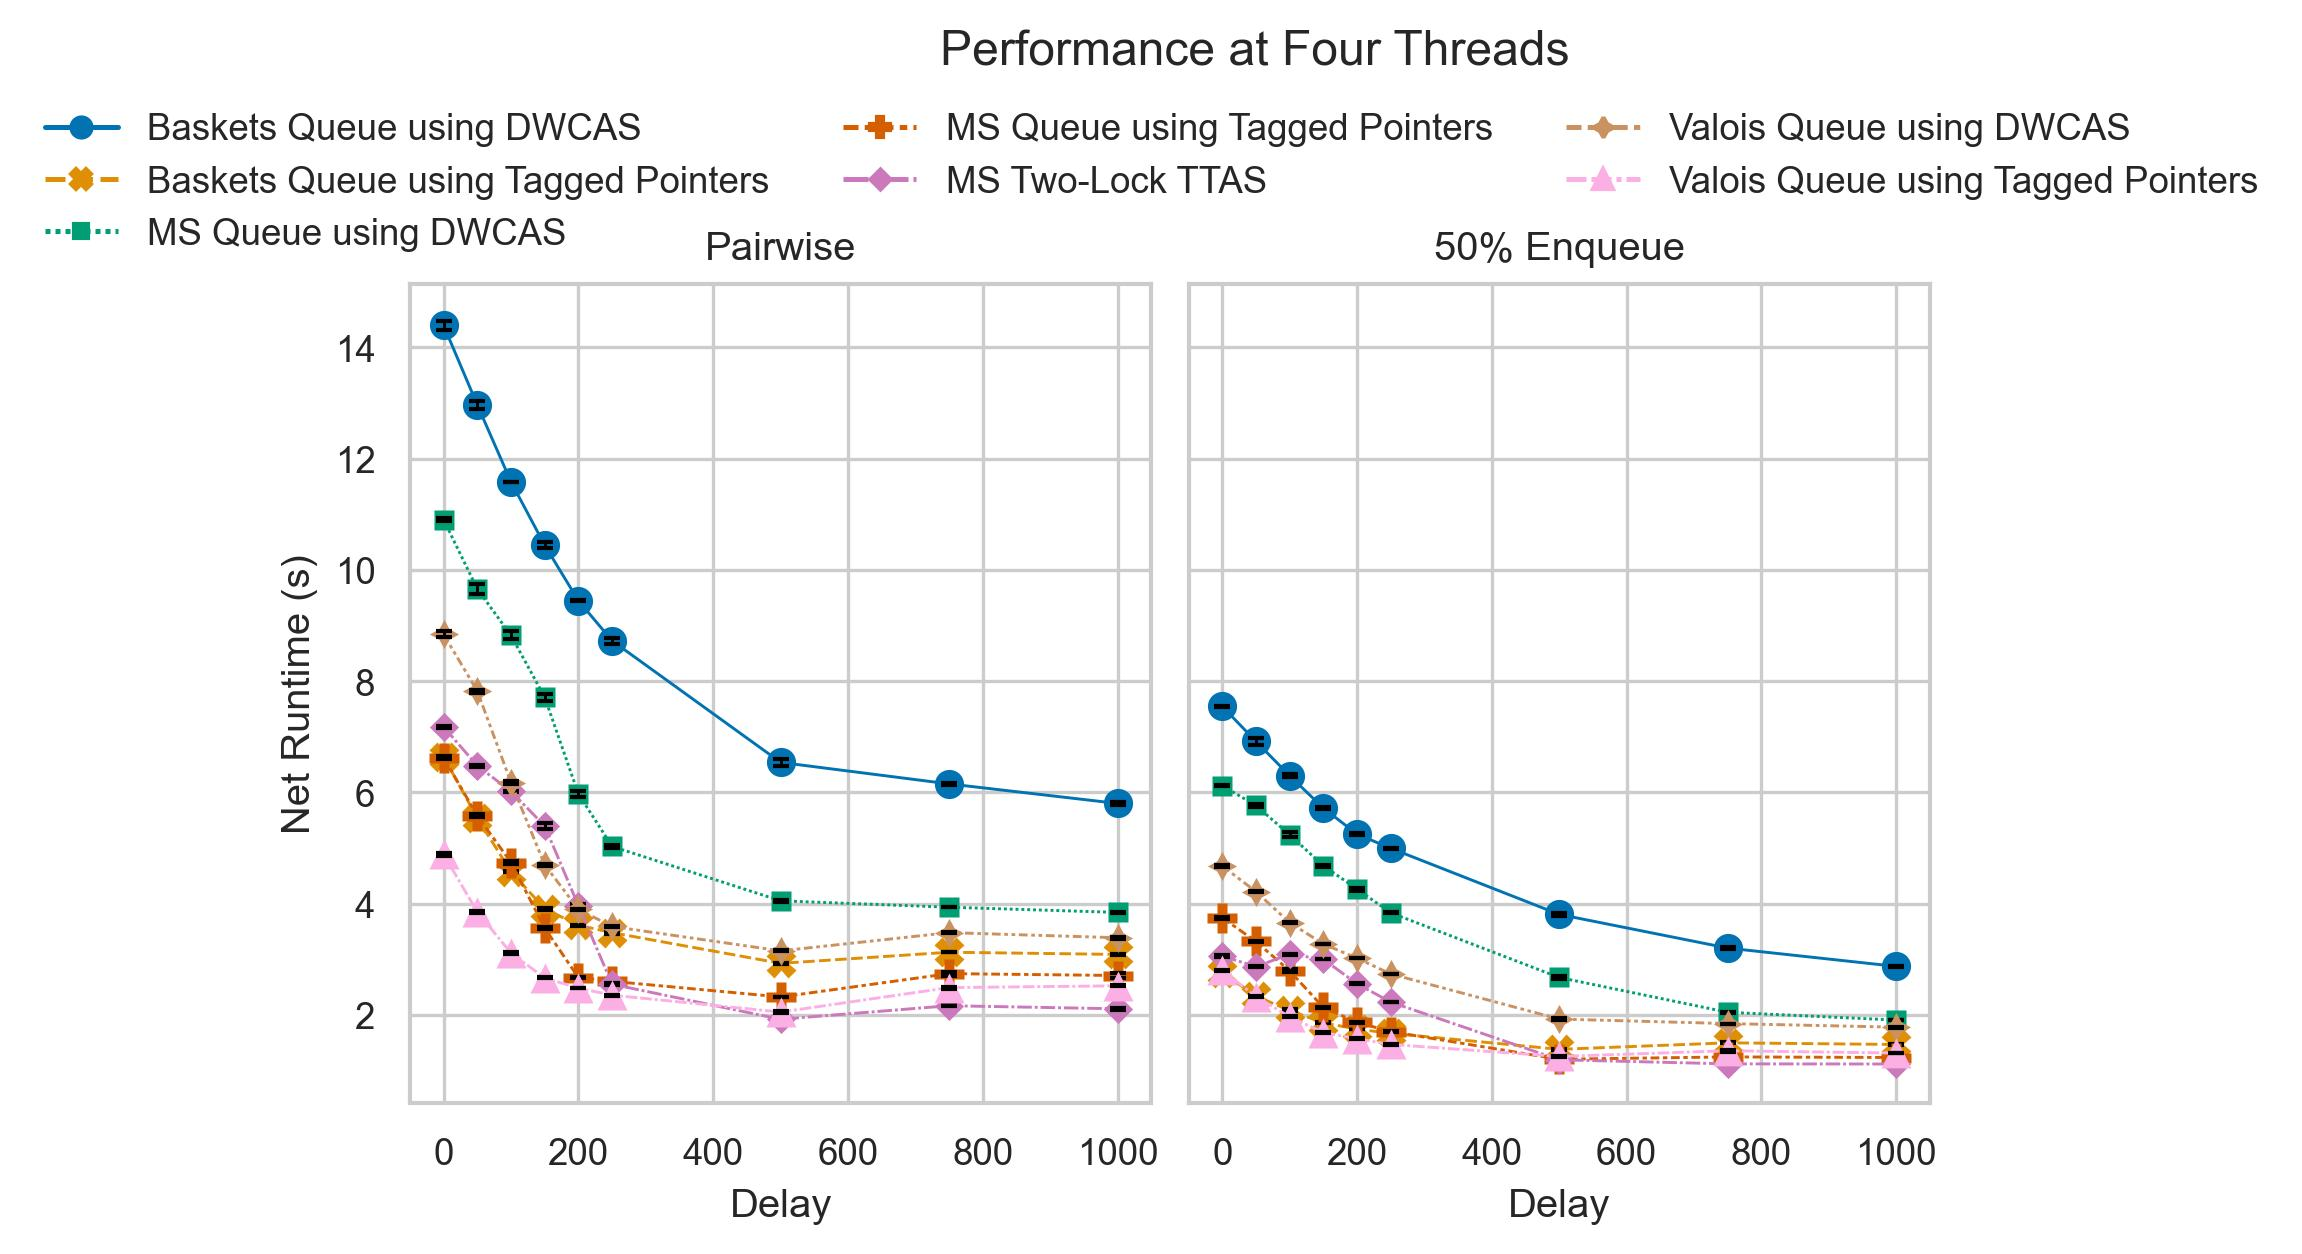
\includegraphics[width=1\textwidth]{images/plots/delay_thread_4.jpg}
    \caption{Pairwise and 50\% Enqueue Benchmarks at four threads.}
    \label{fig:perf_4_thread}
\end{figure}

\begin{figure}[!ht]
    \centering
    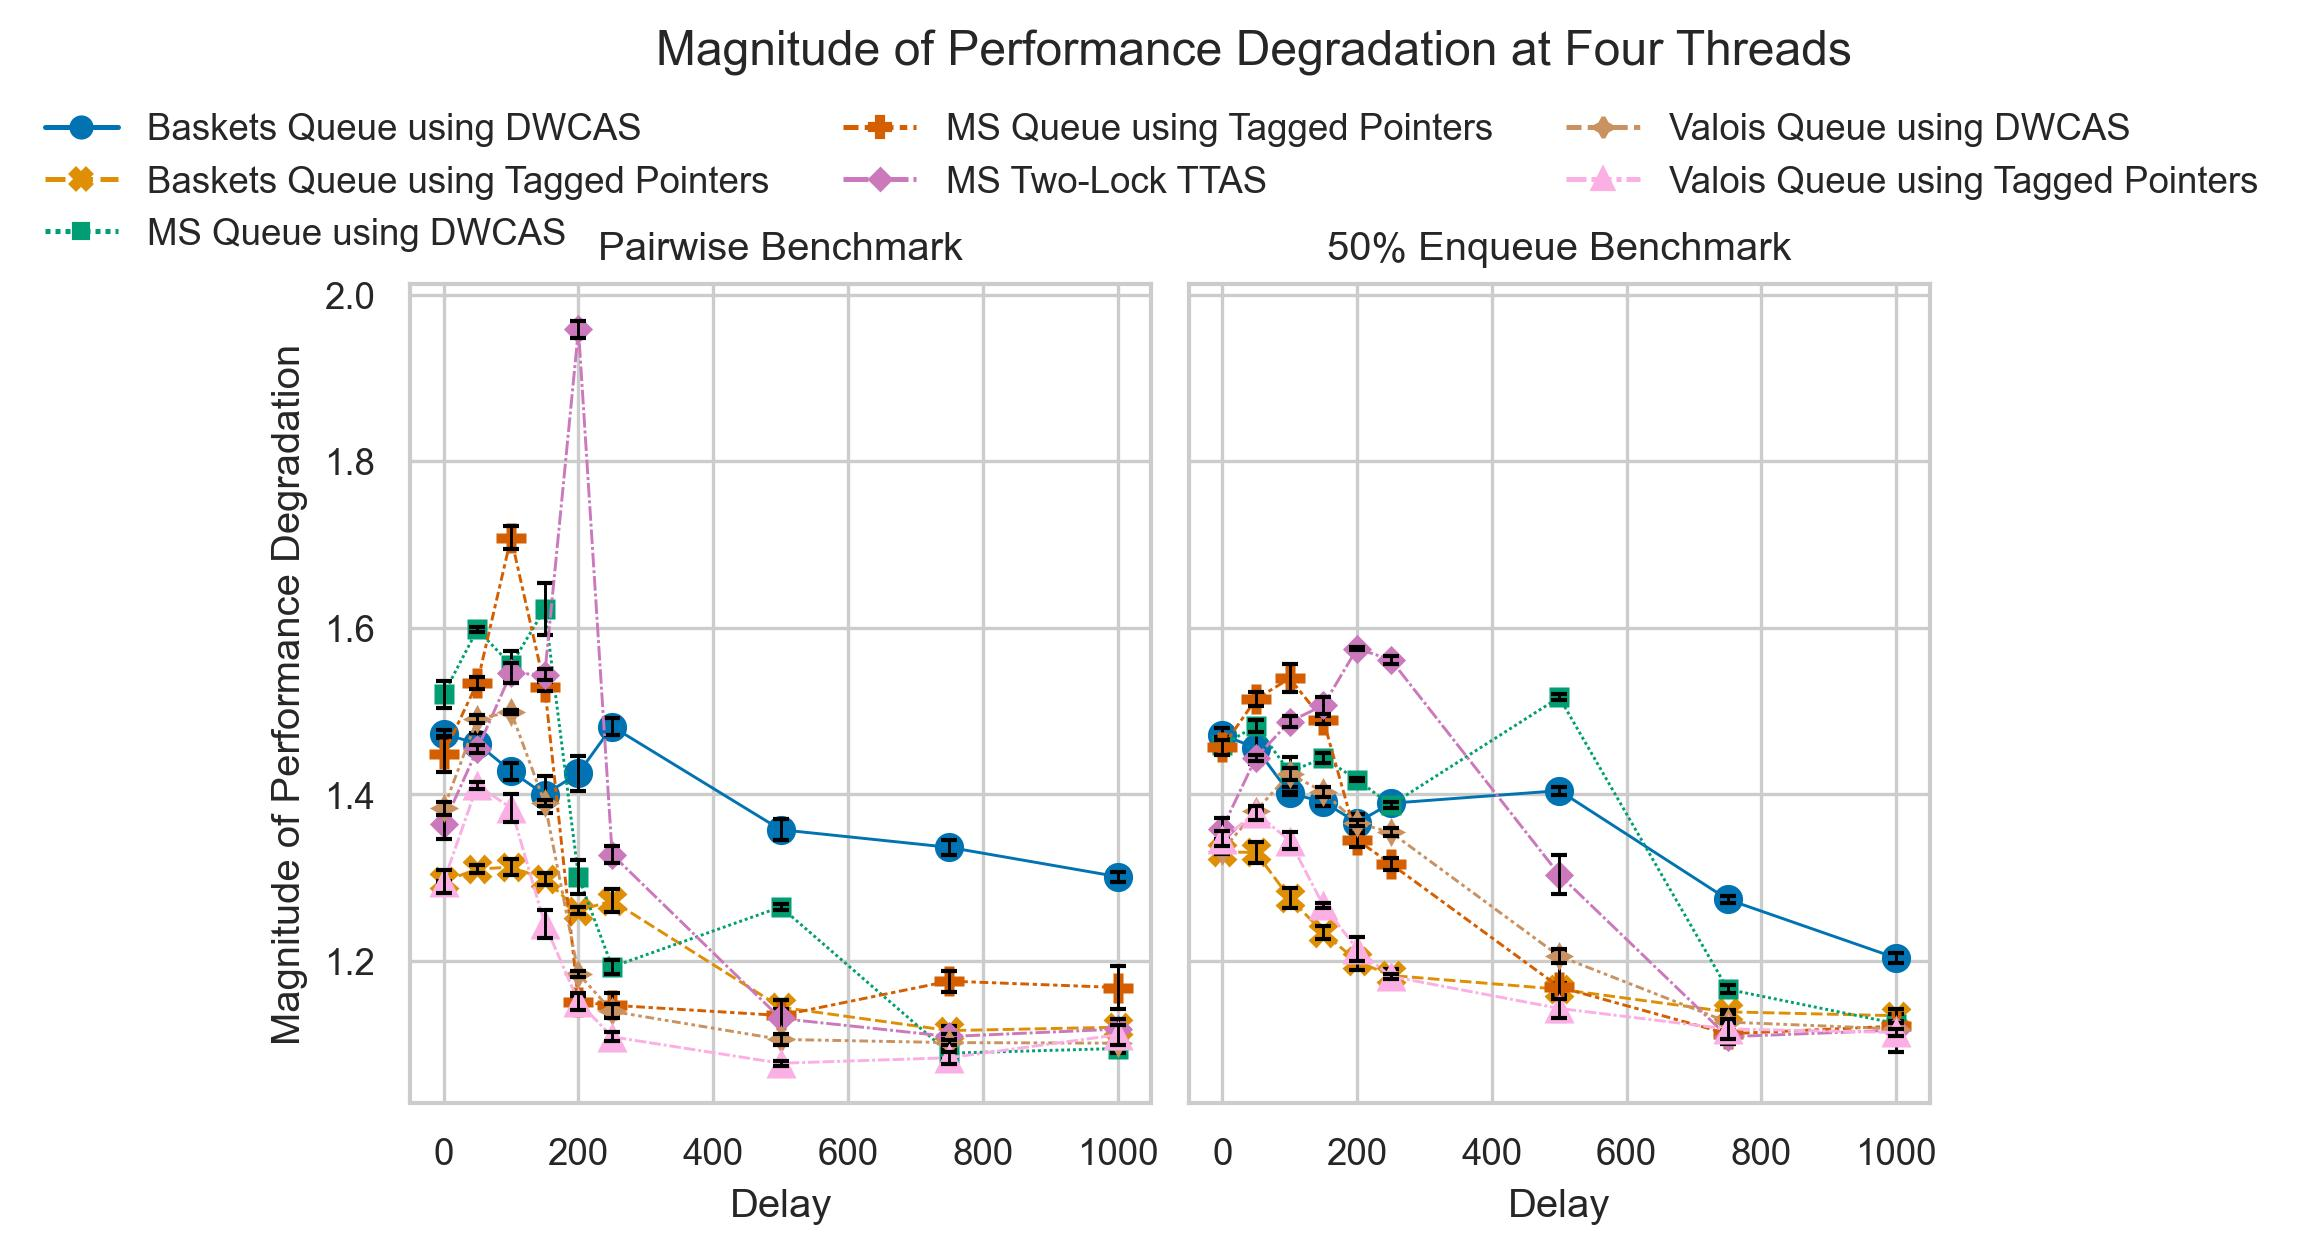
\includegraphics[width=1\textwidth]{images/plots/speedup_3.jpg}
    \caption{Degree of performance degradation at four threads.}
    \label{fig:perf_deg_4_thread}
\end{figure}

\pagebreak

\section{Performance Under Oversubscription}
\subsection{Workload Under Five Threads}
In this study, processors are oversubscribed by pinning more than one process
to each processor, forcing the thread scheduler to increase the frequency of
context-switches.

Figure \ref{fig:perf_deg_5_thread} shows that between 0 and 150 nanoseconds of delay, the
magnitude of performance degradation is a linear function of delay; As delays
greater than 150 nanoseconds are used, performance degradation explodes.
One may hypothesize that the sudden explosion in performance degradation is a result of
the significantly decreased time between context switches; as delay increases, 
the total CPU time available is further reduced.

In the pairwise benchmark, between 0 and 250 nanoseconds of delay, the \emph{Baskets
Queue} and the \emph{MS-Queue} are at most
\textbf{47.045\%} and \textbf{60.604\%} faster than the \emph{two-lock queue};
Between 500 and 1000 nanoseconds, the \emph{two-lock queue} is at most \textbf{3.351\%}
faster than the baskets queue.

Similar to the trends observed in section \ref{sec:workload_four_threads}, the \emph{Baskets
Queue} significantly outperforms the \emph{MS-Queue} (by at most \textbf{53.645\%}) only
in the \emph{50\% Enqueue Benchmark}. This repeating pattern shows that the performance of the
\emph{Baskets Queue} is heavily dependent on the utilization of the baskets mechanism.

\begin{figure}[!ht]
    \centering
    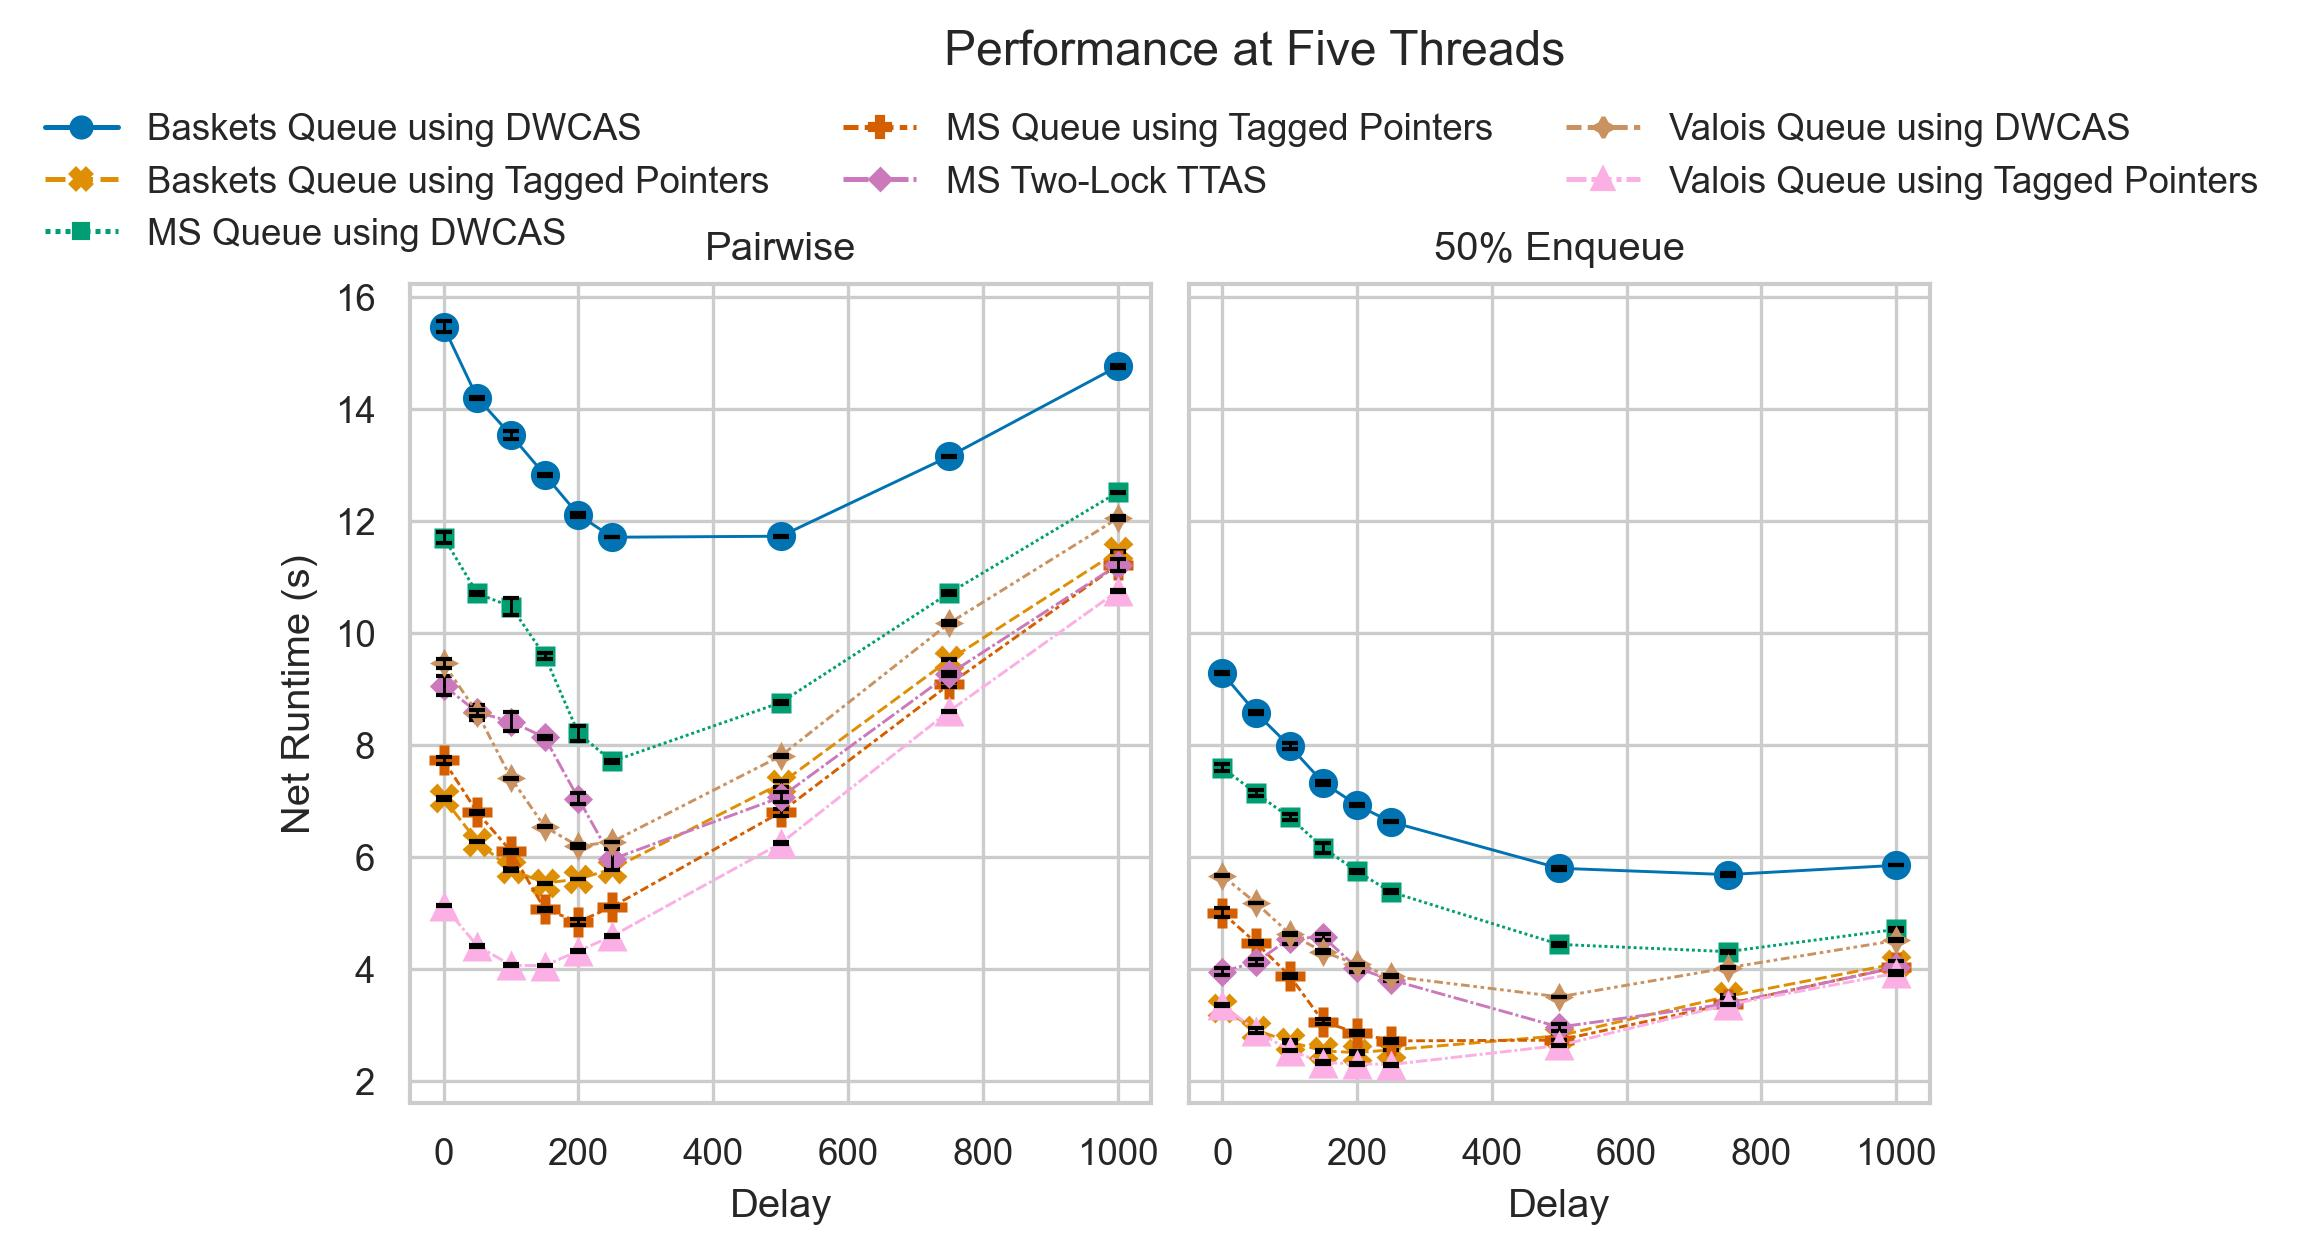
\includegraphics[width=1\textwidth]{images/plots/delay_thread_5.jpg}
    \caption{Pairwise and 50\% Enqueue Benchmarks at five threads.}
    \label{fig:perf_5_thread}
\end{figure}

\begin{figure}[!ht]
    \centering
    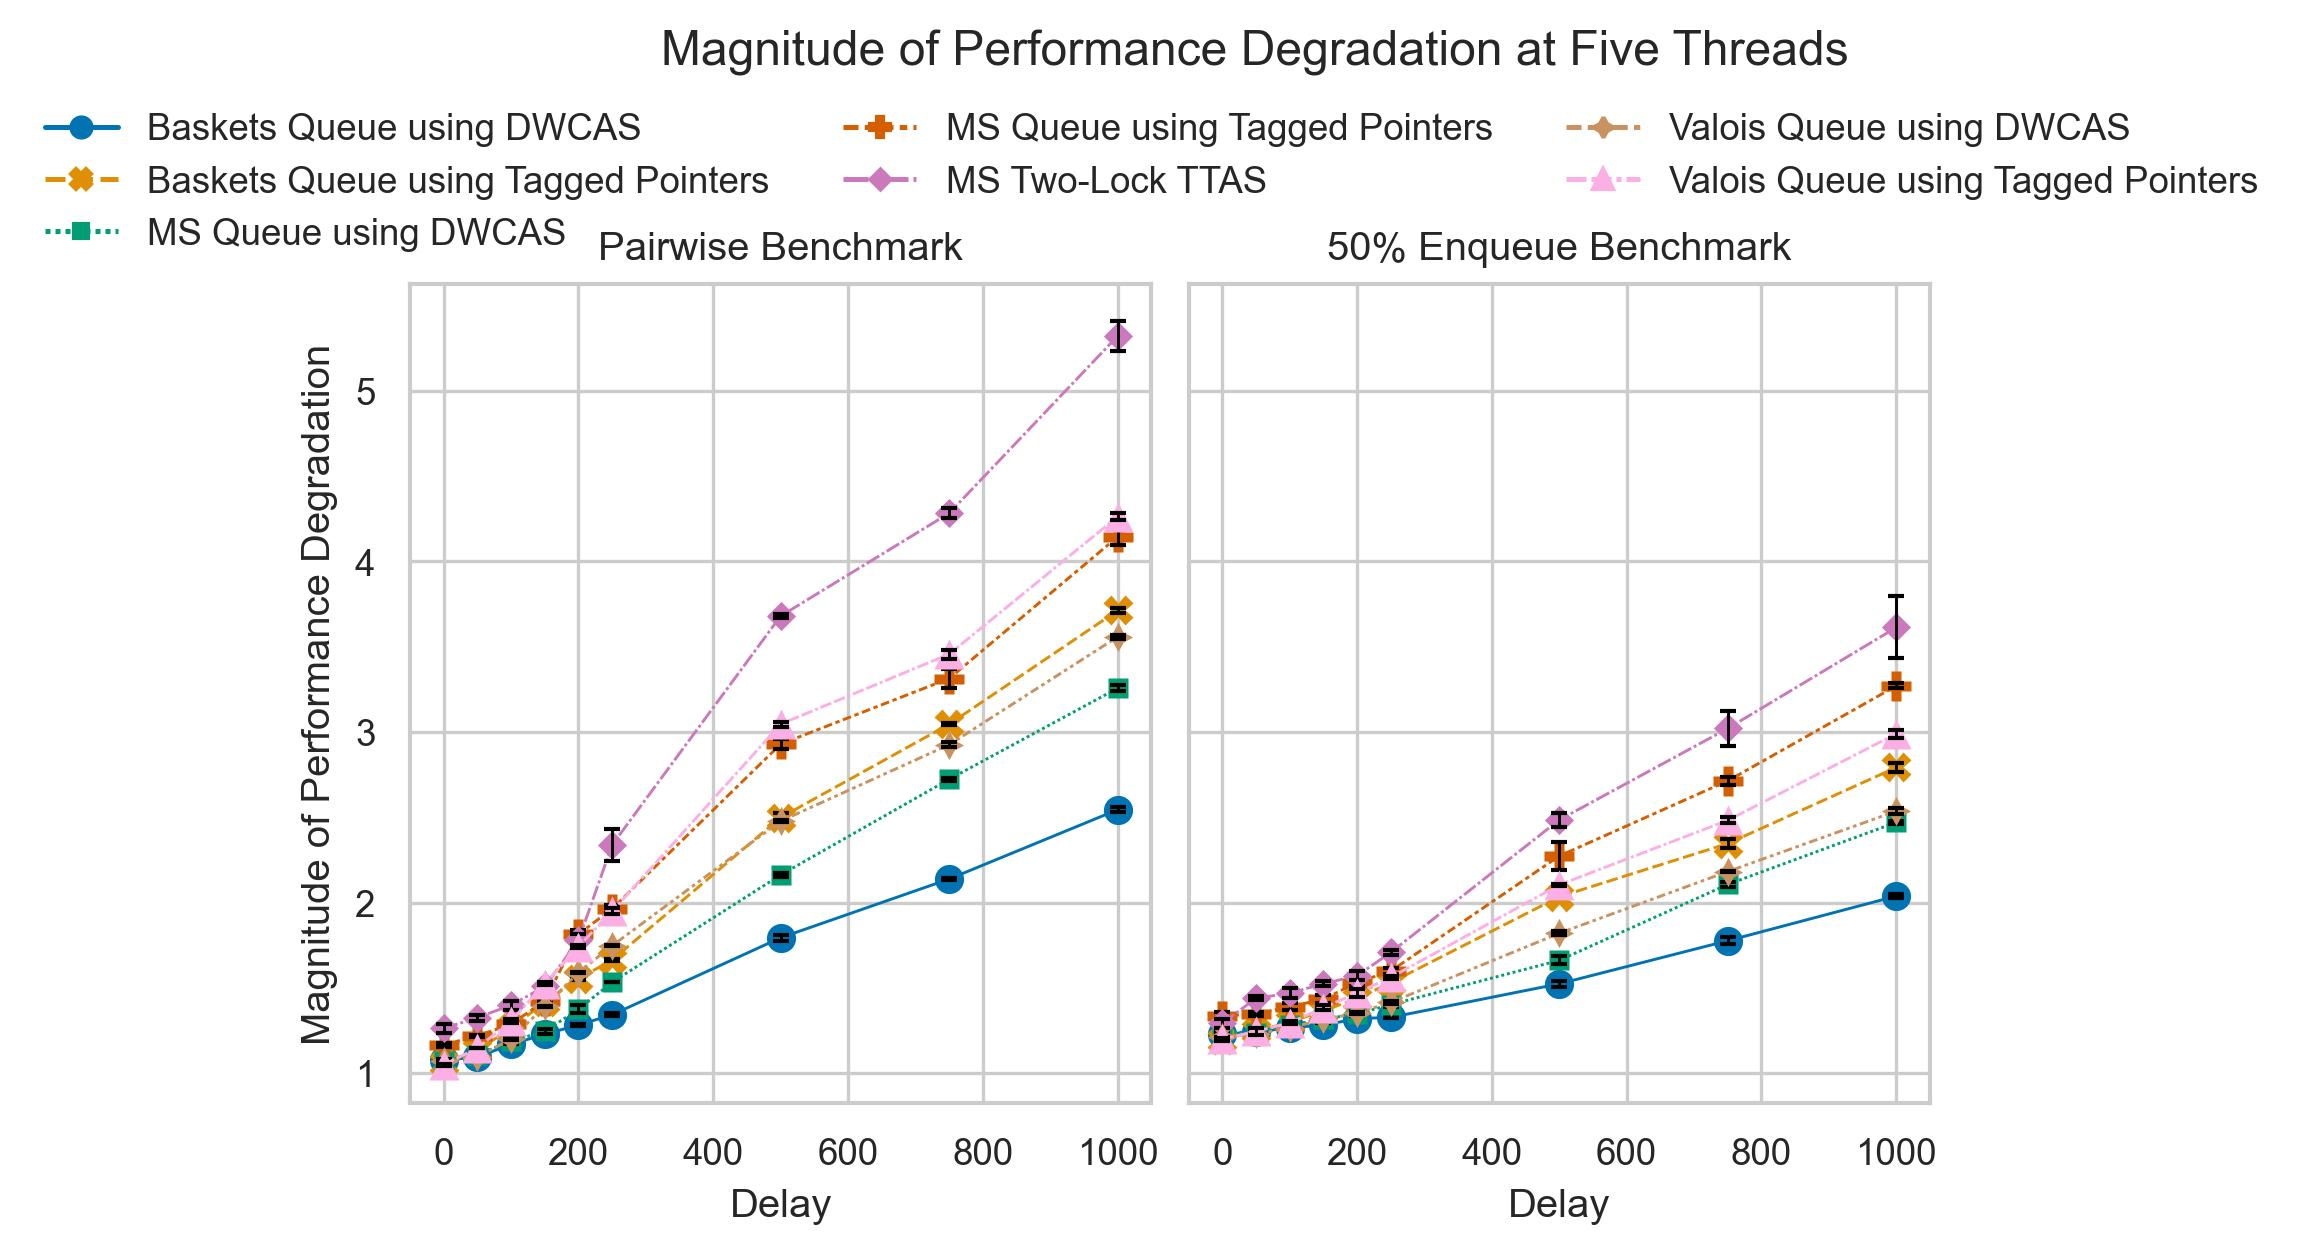
\includegraphics[width=1\textwidth]{images/plots/speedup_4.jpg}
    \caption{Degree of performance degradation at five threads.}
    \label{fig:perf_deg_5_thread}
\end{figure}

\section{Six Threads and Above}
At six threads, the non-blocking queues significantly outperform the \emph{two-lock}
queue at every delay. This trend repeats itself up to 12 threads, with the
degree at which the non-blocking queues outperform the \emph{two-lock queue}
increasing at every thread; the degree at which the \emph{baskets queue} outperforms
the \emph{MS-Queue} also grows with every thread.
% \section{Biases and Threats to Validity}
% \paragraph{Artificiality of Workloads}
% In \citep{gregg2014systems}, \citeauthor{gregg2014systems} claims that
% \emph{micro-benchmarks} (type of benchmark adopted in this study) produces
% artificial workloads, rendering results which are  solely obtained under
% various assumptions. Results obtained in this study represent the concurrent
% queues, whose operations are separated by fixed delays, inside a ``clean-room''
% environment. Realistic workloads seldom follow such rigid patterns, making the
% results' validity under real-world scenarios undetermined.

% \paragraph{Impact of Consumer Grade CPUs on Performance}
% For the scope of this study, cutting-edge hardware, similar to that used in
% prior art, is inaccessible. Unfortunately, over-subscription of processors
% is required to gather enough an acceptable amount of data, making it
% impossible to reproduce trends solely attainable from low-degrees of over-subscription. At
% best, the resources accessible to the study may only produce
% highly-multiprocessed workloads.
